% TeX'ing this file requires that you have AMS-LaTeX 2.0 installed
% as well as the rest of the prerequisites for REVTeX 4.0
%
% See the REVTeX 4 README file
% It also requires running BibTeX. The commands are as follows:
%
%  1)  latex apssamp.tex
%  2)  bibtex apssamp
%  3)  latex apssamp.tex
%  4)  latex apssamp.tex
%
%\documentclass[prb,showkeys,preprintnumbers,amsmath,amssymb, 11pt]{revtex4}
%\documentclass[preprint,showpacs,showkeys,preprintnumbers,amsmath,amssymb]{revtex4}

% Some other (several out of many) possibilities
%\documentclass[preprint,aps]{revtex4}
%\documentclass[aps, two column, amsmath,amssymb,floatfix]{revtex4}
%\documentclass[showkeys,showpacs,amsmath,amssymb,twocolumn,superscriptaddress,prl]{revtex4-1}% Physical Review B  
\documentclass[aps,prl,reprint,showpacs,floatfix,superscriptaddress]{revtex4-2}

\usepackage{amsmath,amsthm,amssymb}
\usepackage{graphicx}% Include figure files
\usepackage{dcolumn}% Align table columns on decimal point
\usepackage{bm}% bold math
\usepackage{color}
\usepackage{epsfig}
\usepackage{multirow}
\usepackage{mathrsfs}
\usepackage{hyperref}
\usepackage{cleveref}
\usepackage{epstopdf}
\usepackage{subfigure}
\usepackage{autobreak}

%Macros for mathematical notations

\newcommand{\V}[1]{\boldsymbol{#1}} %# vector
\newcommand{\M}[1]{\boldsymbol{#1}} %# matrix
\newcommand{\Set}[1]{\mathbb{#1}} %# set
\newcommand{\D}[1]{\Delta#1} %# \D{t} for time step size
\renewcommand{\d}[1]{\delta#1} %# \d{t} for small increment
\newcommand{\norm}[1]{\left\Vert #1\right\Vert } % norm
\newcommand{\abs}[1]{\left|#1\right|} %abs

\newcommand{\grad}{\M{\nabla}} %gradient
\newcommand{\av}[1]{\left\langle #1\right\rangle } %take average

\newcommand{\sM}[1]{\M{\mathcal{#1}}} %matrix in mathcal font
\newcommand{\dprime}{\prime\prime} % double prime
%\global\long\def\i{\iota}
%\renewcommand{\i}{\iota} %i for imaginary unit
%\renewcommand{\i}{\mathsf i} %i for imaginary unit
\newcommand{\follows}{\quad\Rightarrow\quad} %=>
\newcommand{\eqd}{\overset{d}{=}} %=^d
\newcommand{\spe}[1]{\mathscr{#1}}  %important quantities in mathscr font
\newcommand{\eps}{\epsilon}


\begin{document}
\preprint{Preprint}

\title{Induced Charge Oscillations in Dielectric Confined Quasi-2D Systems}

\author{Xuanzhao Gao}
\email{xz.gao@connect.ust.hk}
\affiliation{Thrust of Advanced Materials, The Hong Kong University of Science and Technology (Guangzhou), Guangdong, China}
\affiliation{Department of Physics, The Hong Kong University of Science and Technology, Hong Kong SAR, China}

\author{Zecheng Gan} \thanks{Corresponding author}
\email{zechenggan@ust.hk}
\affiliation{Thrust of Advanced Materials, The Hong Kong University of Science and Technology (Guangzhou), Guangdong, China}
\affiliation{Department of Mathematics, The Hong Kong University of Science and Technology, Hong Kong SAR, China}

\date{\today}

%%%%% Begin Abstract %%%%%%%%%%%
\begin{abstract}
% Quasi-2D charged systems are attracting much attention because of their potential in future nanodevices. 
% The confined geometry gives rise to new physical phenomenons, but also brings great challenges for computational studies.
% We derive a new method to calculate electrostatic interaction between charged particles under dielectric confinement, and demonstrate that static surface plasmonic waves (SSPWs) can be triggered solely via the substrate permittivity.
% Interestingly, period of the SSPWs can be precisely controlled by structure of the quasi-2D system.
% In Molecular dynamics (MD) simulations, we found that the system are induced to form a lattice-like structure under specific confinements, owing to the oscillatory propriety of SSPWs.
An analytic solution is proposed for the Green's function of dielectric confined quasi-2D systems for which theoretical and simulation investigations are rarely reported due to the difficulty of handling the dielectric mismatch.
Based on the solution, we found that under specific confinements, the induced surface charge of an ion shows to be oscillatory, and its \textit{wavelength} is determined by the permittivity and geometry structure of the system. 
An efficient and accurate algorithm is developed for calculating electrostatic interaction between mobile ions, allowing us to study related physical systems using the molecular dynamics algorithm.
% The numerical results show that spontaneous surface charge oscillations can be triggered solely via the substrate permittivity.
The numerical results show that the ions form lattice-like structures triggered solely via the substrate permittivity, owing to the oscillatory property of the induced surface charge.
\end{abstract}

%%%%% end %%%%%%%%%%%

%%%%% AMS/PACs/Keywords %%%%%%%%%%%
%\pacs{no longer needed}

%\keywords{ }
%%%% maketitle %%%%%
\maketitle

%%%% Start %%%%%%

% merge them into one paragragh about quais-2D charged systems
% Among various long-range systems, quasi-2D charged systems are of great importance and have caught much attention recently because of their huge potential in future nanodevices and advanced materials.
\textit{Introduction.}--Quasi-2D systems refer to systems with nano-sized longitudinal thickness in $z$ direction (usually by confinement), bulk-like and modeled as periodic in transverse~$xy$ directions~\cite{mazars2011long}. 
Rich new collective behaviors arise in such systems, to name a few, polyelectrolyte adsorption and structure~\cite{messina2004effect,yuan2020structure}, ion transport and selectivity~\cite{nishizawa1995metal,cervera2006ionic} so that caught much attention.
Interestingly, most of these effects concern the permittivity, i.e., the \emph{dielectric confinement effect}.
Substrate materials for nanoscale confinement can range from dielectric to metallic, and nowadays, electromagnetic metamaterials, described by permittivities that can take negative values~\cite{veselago1967electrodynamics, smith2004metamaterials} under excitation by electromagnetic waves of specific frequencies.
Great efforts have been made to develop negative permittivity materials at very low frequencies~\cite{cheng2017tunable, xie2022recent, xu2020polyaniline}, and recent work has shown that negative static permittivity can be reached in a wide range of materials, such as metals~\cite{kana2016thermally}, quasi-2D crystals~\cite{nazarov2015negative}, nano-particle~\cite{shulman2007plasmalike} and polymeric systems~\cite{yan2013negative}.


For electrolytes/polymers near a \emph{single} dielectric substrate, recent calculations have revealed that the dielectric surface effect can considerably deviate the systems from bulk behaviors, such as ion transport~\cite{antila2018dielectric}, polymer brush structure~\cite{yuan2020structure} and pattern formation in dipolar films~\cite{wang2019dielectric}, especially when permittivity of the substrate is negative.
Unfortunately, the addition of a second dielectric substrate to form dielectric confinement in computer simulations is far from direct-forward: simulation techniques~\cite{arnold2002electrostatics, de2002electrostatics,tyagi2007icmmm2d,fernandez2010collection,jadhao2012simulation,zwanikken2013tunable,fahrenberger2014computing,dos2017simulations,yu2018plasmonic,liang2020harmonic,yuan2021particle,maxian2021fast} have made significant progress over the past decades, but proper treatment of the dielectric confinement effect with satisfactory accuracy and efficiency remains challenging.

% % In this article I think we may discuss less about MD result.
% Nevertheless, in terms of the spontaneous symmetry breaking (SSB) phenomena, much existing study focuses on purely 2D and 3D systems~\cite{levin:PRL:2008,joyce2011quasistationary,pakter2018nonequilibrium}, far less is known about quasi-2D.
% For bulk electrolytes or neutral plasma, it is well-known that the Coulomb potential can be dynamically screened by surrounding countercharges, leading to effectively short-range interacting particle systems~\cite{huckel1923theory}. 
% The situation becomes very different in quasi-2D charged systems: their reduced symmetry (i.e., the nano-sized confinement) weakens the electrostatic screening, and correlation effect can become much more important. Clearly, this is quasi-2D specific, where simplified 2D description would fail. 
% Yet, to the best of our knowledge, no SSB phenomena have been reported in suspension of charge- and size-symmetric, overall-neutral particle systems under dielectric confinement, without any external fields.


% Here I would like to add a section about surface plasmonic waves
% For systems with dielectric mismatch, surface plasmonic waves (SPWs) may arise from the collective oscillations of the electrons as a particular type of electromagnetic wave at the interface, for example, between metal and dielectric~\cite{zhang2020terahertz, polo2011surface}.
% Traditionally, SPWs are excited by electromagnetic waves and then propagate along the surface.
% Because of the strong interaction between photons and electrons, the field is confined near the surface and interacts strongly with the material, so that can be widely used in communications and photonic circuits~\cite{wu2003terahertz, tao2008metamaterial, o2008thin}.
% Recent work has shown that negative static permittivity can be reached in a wide range of materials, such as metals~\cite{kana2016thermally}, quasi-2D crystals~\cite{nazarov2015negative}, nano-particle~\cite{shulman2007plasmalike} and polymeric systems~\cite{yan2013negative}.
% making it possible for SPWs to be excited by a static field source.

% Here I rewrite this paragraph and changed the main point the SSPWs, and treat MD result as a usage of SSPWs
In this letter, we develop a method to calculate electrostatic interaction for charged particles in quasi-2D systems under dielectric confinement.
By properly renormalization, our method can calculate the electrostatic interaction in meta-material confined systems.
We further develop a lattice summation formula for simulating charged particles in such systems, and its spectral convergence allows us to calculate the polarization field efficiently. 
Applying our method, we show that induced surface charge oscillations arise on substrates under metamaterial confinements.
The effect of surface polarization on ionic distributions is further explored through molecular dynamic (MD) simulations of a prototypical charge- and size-symmetric binary mixture of particles described by the primitive model~\cite{mcmillan1945statistical}, which demonstrate that, the polarization charge on the surface can induce the system to form lattice-like structures and size of the lattice cell can be controlled by tuning the permittivity and thickness of the system.
% As explained below, we attribute the lattice formation to the oscillatory properties of SSPWs.


% In this letter, we develop a new lattice summation formula for the Green's function in simulating charged particles under dielectric confinement, its spectral convergence allows us to efficiently calculate the polarization field. 
% Through computer simulations of a prototypical charge- and size-symmetric binary mixture of particles described by the primitive model~\cite{mcmillan1945statistical},
% we demonstrate that broken symmetries arise spontaneously due to the dielectric confinement effect alone.
% Moreover, we discover that the substrates permittivity can even qualitatively alter the degree of SSB in longitudinal and transverse dimensions, forming charge-separated interfacial liquids and correlated-clusters. 
% Noteworthy is that all the SSB phenomena reported here actually require the presence of \emph{two} dielectric substrates, we attribute this to the complicated multiply scattered polarization field due to the layered dielectric confinement structure.

% The Green's function~$G(\V r; \V r^\prime)$ for a doubly-periodic, dielectric confined geometry is described by the Poisson's equation,
% \begin{equation}
% 	-\grad\cdot\left[\epsilon(\V r) \grad G(\V r; \V r^\prime)\right] = \sum_{\norm{\V m}=0}^{+\infty} \d(\V r - \V r^\prime_{\V m} )\;,\label{eq:Green4Poisson}
% \end{equation}
% where~$\V r,~\V r^\prime\in \begin{bmatrix} 0, L_x\end{bmatrix}\times\begin{bmatrix} 0, L_y\end{bmatrix}\times\begin{bmatrix} 0, L_z\end{bmatrix}$ are the target and source locations within the simulation box,~$\V r^\prime_{\V m} = \V r^\prime + m_xL_x\hat{\V x}+m_yL_y\hat{\V y}$ accounts for the periodic replicas along~$x$ and~$y$ directions, with~$\V m = \begin{pmatrix} m_x, m_y\end{pmatrix}$ the 2D lattice vector,~$m_x, m_y \in \mathbb Z$.
% Importantly,~$\epsilon(\V r)$ is the material-specific, spatially varying dielectric constant, as is depicted in Fig.~\ref{fig:ICM}. 
% Finally, we have the dielectric interface conditions, i.e., the continuity of~$G(\V r; \V r^\prime)$ and~$\epsilon(\V r)\partial G(\V r; \V r^\prime)/\partial z$ across~$z= 0$ and~$L_z$, and the free-space boundary condition (FBC) as~$z\to\pm\infty$. 
% Note that for charges under dielectric confinement, proposing the proper FBC needs careful considerations so as to make it physically well-defined, which we will clarify later.
\begin{figure}[htbp]
	\centering
	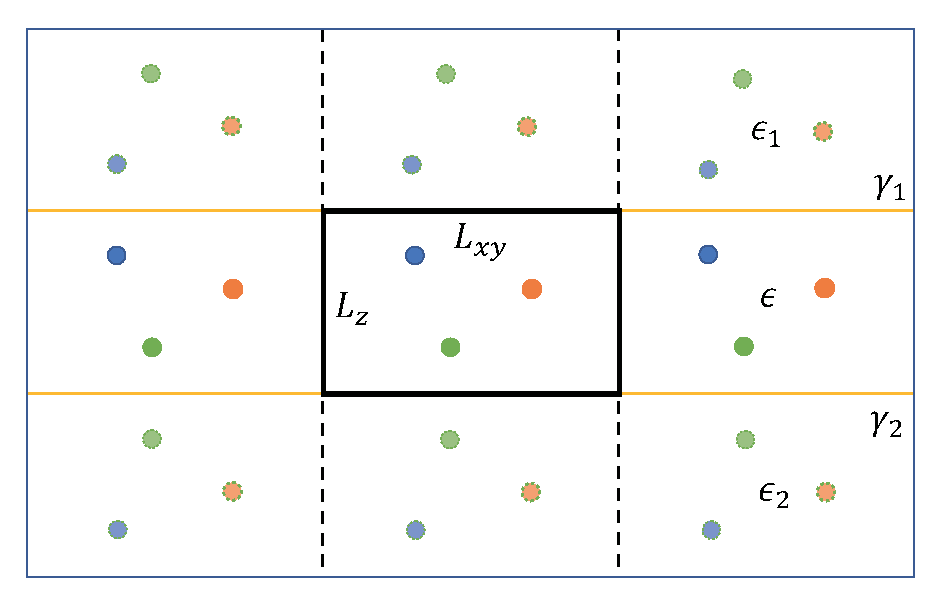
\includegraphics[width=0.45\textwidth]{figs/fig1.pdf}
	\caption{
		Schematic depiction of a quasi-2D charged system, the dielectric confinement effect is illustrated from the Image Charge Method (ICM) viewpoint. The middle layer represents the solvent medium with dielectric permittivity~$\epsilon$; the upper and lower layers represent the substrate with dielectric permittivity~$\epsilon_1$ and~$\eps_2$, respectively. Colored circles surrounded by solid lines are real charged particles of the doubly-periodic system, while those surrounded by dotted lines are image charges reflected by dielectric interfaces in~$z$.
		\label{fig:ICM}
	}
\end{figure}


% To gain insight into the role of dielectric confinement in quasi-2D systems, we start our discussion with the classic Image Charge Method (ICM). 
% Consider a point charge~$q$ located in a medium with dielectric constant~$\epsilon$ and is near a single planar substrate with dielectric constant~$\epsilon_s$, the polarization potential can be equivalently expressed as the Coulomb potential generated by an image charge located with mirror-symmetry, and magnitude~$q_{\mathrm {img}}=\gamma q$.
% The dimensionless coefficient~$\gamma = (\eps - \eps_s)/(\eps + \eps_s)$ quantifies the strength of polarization, and in the following discussion, we will keep~$\eps = 1$ unchanged when tuning~$\gamma$. 
% Usually,~$\abs{\gamma}\leq 1$ for materials with positive permittivity, but the upper bound can be further lifted for metamaterials because of their stronger polarizability, characterized by negative static permittivity values~\cite{urzhumov2012magnetic, coffey2012magnetic}, so that that~$\gamma$ can be tuned into a much more comprehensive range.

\textit{The model.}--The geometry of the dielectric confined quasi-2D systems modeled for simulations is shown in Fig.~\ref{fig:ICM}, which is doubly periodic in the transverse direction and finite in the longitudinal direction with edge length of~$L_x$,~$L_y$ and~$L_z$.
All charged particles are distributed between the dielectric substrates with dielectric permittivity~$\eps_1$ and~$\eps_2$, and immersed in solvent with dielectric permittivity~$\eps$.
Based on the ICM, the dimensionless coefficient reflection rate, ~$\gamma_1$ and ~$\gamma_2$ given by~$(\eps - \eps_i)/(\eps + \eps_i)$, quantify the strength of polarization.
Then Green's function of Poisson's equation in such systems can be constructed via a multiple reflection process, resulting in an infinite image charge series, schematically illustrated in Fig.~\ref{fig:ICM}.
Note that when~$\abs{\gamma_1 \gamma_2}\leq 1$, the image reflection series is convergent; but when~$\abs{\gamma_1 \gamma_2}>1$, it will be \emph{divergent} and thus the reflective ICM approach would fail. 
Due to this divergence difficulty, current simulation studies in the~$\abs{\gamma}\geq 1$ regime is still limited to a single dielectric substrate~\cite{wang2019dielectric}.
Our new approach overcomes this divergence issue via a proper renormalization strategy, which allows us to extensively explore the dielectric confinement effect in all possible~$\gamma$ regimes, especially the less explored scenario of metamaterial substrates with static negative permittivity.


Green's function~$G(\V{r},\V{s})$ for Poisson's equation of a dielectric confined quasi-2D system is given by
\begin{equation}
    -\grad\cdot\left[\eta(\V r) \grad G(\V{r},\V{s})\right] = 4 \pi \d(\V r - \V s )\;,\label{eq:Green4Poisson}
\end{equation}
where~$\V{r}$,~$\V{s}$ are target and source locations under the confined geometry.
Importantly,~$\eta(\V r) = \eps(\V{r}) / \eps$ characterizes the relative dielectric function which is piecewise constant.
Here,~$\eps(\V{r})$ is the material-specific, spatially varying dielectric constant, defined as 
\begin{equation}
    \eps(\V{r}) = \left\{
    \begin{array}{cc}
        \eps_1,~ & z > L_z \\
        \eps,~ & 0 \leq z \leq L_z \\
        \eps_2,~ & z < 0
    \end{array}
    \right. \;,
\end{equation}
as is depicted in Fig.~\ref{fig:ICM}. 
Finally, we have the dielectric interface conditions, i.e., the continuity of~$G(\V r, \V s)$ and~$\epsilon(\V r)\partial_z G(\V r, \V s)$ across~$z= 0$ and~$L_z$, and the free-space boundary condition (FBC) as~$z\to\pm\infty$. 
Note that for charges under dielectric confinement, proposing the proper FBC needs careful consideration to make it physically well-defined, which we will clarify later.
In the following discussion, we set~$\eps = 1$ and~$\eps_1 = \eps_2 = \eps'$ so that~$\gamma_1 = \gamma_2 = \gamma$, by changing~$\eps'$, we vary~$\gamma$ from~$-10$ to~$10$.
Such systems can be achieved via tuning permittivity of the substrates material.
For example, the permittivity of VO$_2$ will reach about~$-14$ at about~$350$K~\cite{kana2016thermally}, so that by choosing solvents with permittivity of~$11.4$ or~$17.1$ (e.g. organic solvents), the proposed~$\gamma$ can be achieved.

\begin{figure}[htbp]
	\centering
	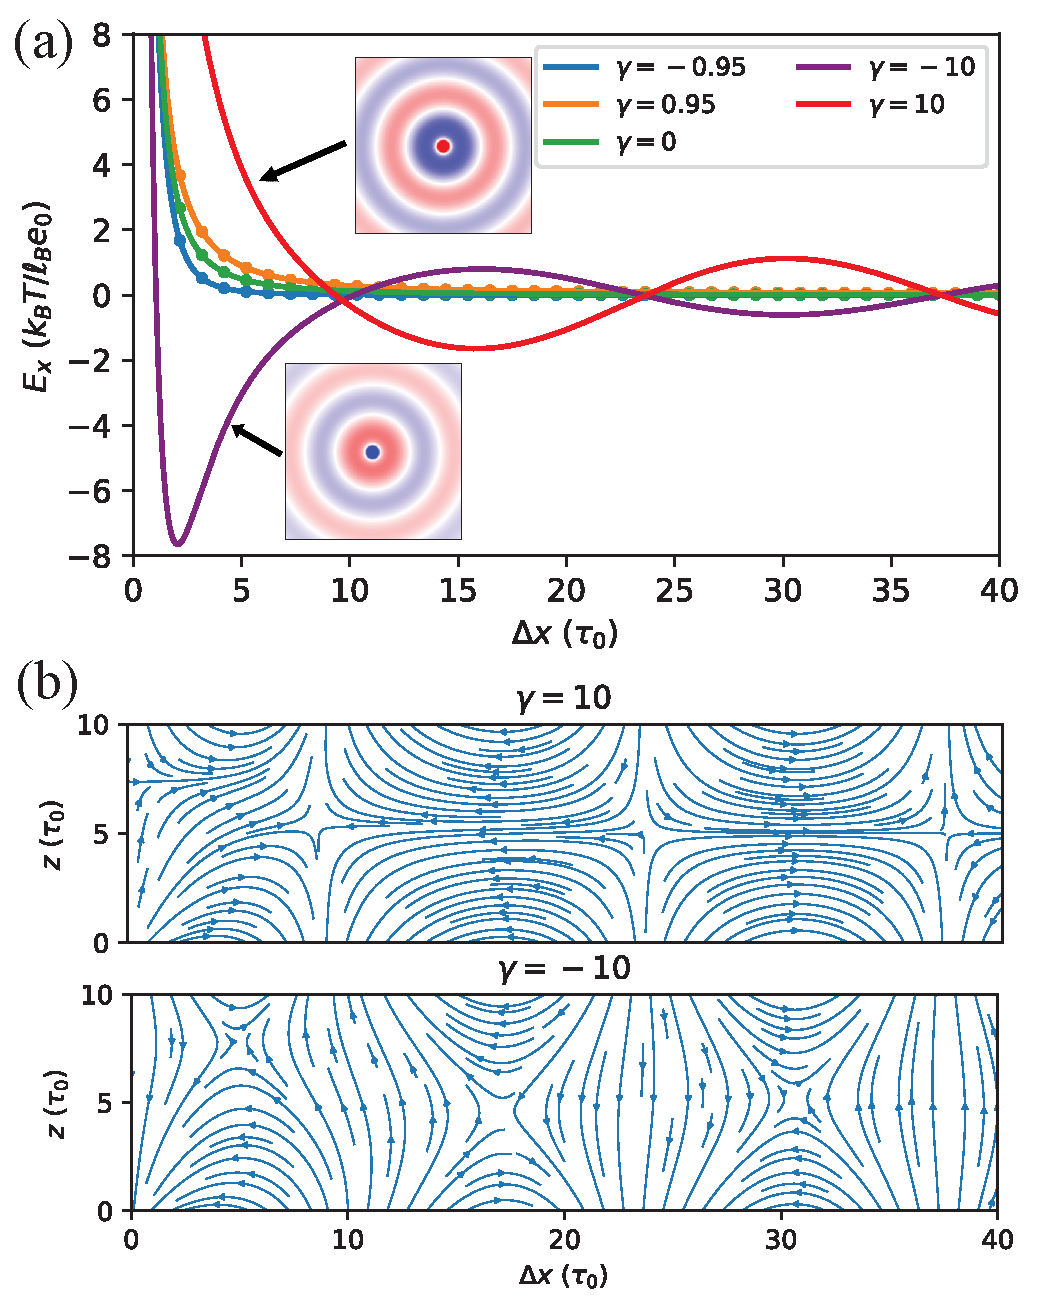
\includegraphics[width=0.45\textwidth]{figs/fig2.pdf}
	\caption{
        Electric fields in~$x$ by a cation with valence~$\nu = 1$ fixed at~$(z = \tau_0)$ confined by a pair of dielectric substrates at~$z = 0$ and~$10 \tau_0$ are shown in (a) and the sub-figures represent surface charge density on the lower substrates.
        For~$\gamma = \pm 10$ cases, the corresponding field lines are plotted in (b).
        % The numerical fitting results of the dispersion relation are shown in (c), where the dots are sampling points, and dashed lines are fitting results.
		\label{fig:force_x}
            }
\end{figure}

% Here the discussion about force between charges should be placed later, after the solution for one point charge is given
\textit{Oscillatory single particle field.}--The dielectric confinement effect turns out to be physically attractive even when only one charged particle is present. 
In Fig.~\ref{fig:force_x} (a), we plot the electric field in~$x$ of a cation with valence~$\nu = 1$ at~$(x_0, y_0, \tau_0)$ in a quasi-2D system with thickness of~$10 \tau_0$, as a function of distance from the cation~$\D x = x - x_0$, and the confinements are characterized by reflection rate~$\gamma$.
The field is defined as~$ - \nu \ell_B \partial_x G(\V r, \V{r_0})$, with~$G(\V r, \V{r_0})$ given later in Eq.~\eqref{eq:G_pv}, and the coupling parameter~$\ell_B = e^2 / (4 \pi \eps_0 \eps k_B T)$ is the Bjerrum length of the solvent with the elementary charge~$e$, the vacuum permittivity~$\eps_0$, the Boltzmann constant~$k_B$, and temperature~$T$.
For~$\abs{\gamma} < 1$ cases, as shown by blue and orange lines in Fig.~\ref{fig:force_x} (a), the Coulomb effect is enhanced or reduced because of polarization on the surface comparing to~$\gamma = 0$ case, respectively.
It also shows that our method agrees well with ICM, its results are shown as dots in Fig.~\ref{fig:force_x} (a).
However, when~$\abs{\gamma} > 1$, the result is highly non-trivial, as shown by purple and red lines.
The short-range interaction behave as strongly repulsive or attractive when~$\gamma = 10$ or $-10$, respectively, which can be regarded as an extension of that in~$\gamma < 1$ cases.
Interestingly, the field did not decay to~$0$ but shows to be oscillatory in the transverse direction, which is different from previous observations.

Polarization charge on the surface $(z = 0)$ is shown as the sub-figures of Fig.~\ref{fig:force_x}~(a) explain the non-trivial behavior of the field, which is defined as 
\begin{equation}
    \sigma(\V{r}) = \lim_{z \to 0^+} \nu \ell_B \eps_0  \left( 1 - \frac{\eps}{\eps'} \right) \partial_z G(\V{r}, \V{r_0})\;,
\end{equation}
and the field lines in the~$xOz$ plane generated by the surface charge are shown in Fig.~\ref{fig:force_x}~(b).
These self-consistent results may give an qualitative explain to the non-trivial behavior of the field.
At the center, the strong surface charge dominate in both cases as expected, so that even reverse the field.
For the long-range field, the surface charge also oscillates along the transverse direction, caused by the intense polarization at the center and enhanced by the bi-surface reflection, generating corresponding fields.
The oscillatory field here has a similar structure to that of a surface plasmonic wave but have a different origin, it arise from the reflection by the substrates.
It is also shown that for~$\gamma > 0$ and $\gamma < 0$ cases, polarize charge and field in~$z$ on the opposite substrates are anti-symmetric and symmetric, respectively, which is self-consistent with the definition of~$\gamma$.

More interestingly, for both cases, the \emph{wavelength}~$\lambda$ of the field, defined as two times the distance between nearby zero points, is only related to resonance frequency of the system, given by
\begin{equation}\label{eq:k0}
    k_0 = \frac{\ln{\gamma_1 \gamma_2}}{2 L_z}\;,
\end{equation}
which will be further discussed below, and via numerical calculation we found they have a simple relation
\begin{equation}\label{eq:wavelength}
    \lambda \cdot k_0 \sim 2 \pi \;.
\end{equation}
We find that Eq.~\eqref{eq:wavelength} is highly robust, the relation is irrelevant to~$\V{r}$,~$\V{r}_0$,~$\gamma$ or $L_z$ once~$k_0$ is given, as shown in Fig.~\ref{fig:k_wavelegth}, which means that the effect can be accurately controlled by adjusting~$k_0$.
% Based on the reasons above, we consider the effect as a \emph{static} surface plasmonic wave, for it shows remarkable similarities to SPWs, and can be excited by a stationary field source.
% We take different~$L_z$, i.e.~$10$ and~$15$, and then change the value of~$\gamma$ to tune~$k_0$.
% For each point, we randomly generated~$z$ and~$z_s$ as the position of the source charge and the test charge, respectively. Then we move the test charge along~$x$ axis, and take an average on distance between zeros points of~$E_x$.
% The numerical results show that the relation is highly robust and has no relation to position of the ions.

\begin{figure}[htbp]
    \centering
    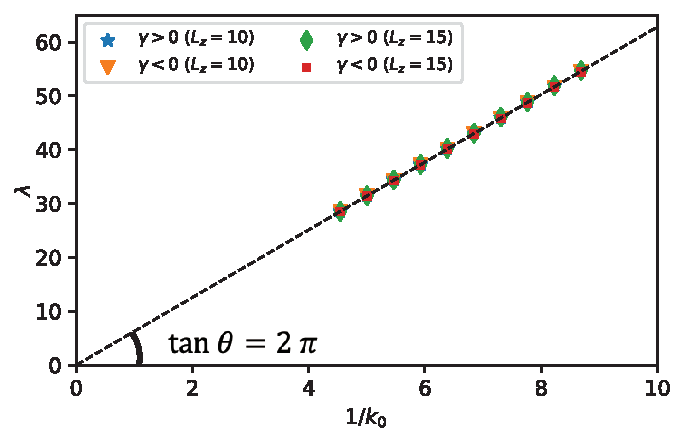
\includegraphics[width=0.45\textwidth]{SIfig/k_wavelegth.pdf}
    \caption{
        Numerical results for relation between~$k_0$ and~$\lambda$.
        The system parameters, $\gamma$ and~$L_z$, are changed to tune~$k_0$.
        For each point in the figure, we calculated the interaction between a pair of particles with randomly generated position in~$z$ as a function of~$\D \rho$.
        Then the average distance between zero points of~$E_x$ is taken as~$\lambda / 2$.
    }
    \label{fig:k_wavelegth}
\end{figure}


Eq.~\eqref{eq:Green4Poisson} can be solved directly because of the special geometry.
To start, one applies plane wave expansion on both sides of the equation so that the Green's function can be expressed as 
\begin{equation}\label{eq:G_point_charge}
    \begin{split}
        G(\V{r},\V{s}) & = - \frac{1}{\pi} \iint_{\mathbb{R}^2} g(k, z, z_s) e^{-i \V{k} \cdot \Delta \V{\rho}} \text{d} k_x \text{d} k_y \\
        & = - \int_{0}^{+\infty} 2 g(k, z, z_s) J_0(k \Delta \rho) k \text{d}k\;,
    \end{split}
\end{equation}
where~$\V{k} = (k_x, k_y)$,~$\Delta \V{\rho} = (x - x_s, y - y_s)$.
When~$k>0$, ~$g(k, z, z_s)$ 
% satisfies differential equation and boundary conditions given by
% \begin{equation}\label{eq:g_diff}
%     \begin{split}
%         & \partial_z^2 g(k, z, z_s) - k^2 g(k, z, z_s) = \d (z - z_s)\\
%         & \eps \partial_z g(k, L_z, z_s) + \eps_1 k g(k, L_z, z_s) = 0\\
%         & \eps \partial_z g(k, 0, z_s) - \eps_2 k g(k, 0, z_s) = 0\;.
%     \end{split}
% \end{equation}
% Solution of Eq.~\eqref{eq:g_diff} 
is given as
\begin{equation}\label{eq:g_solution}
    g(k, z, z_s) = \frac{1}{2k} \frac{1}{\gamma_1 \gamma_2 \exp{(-2 k L_z)} - 1} \sum_{i = 1}^{4} \Gamma_l \text{e}^{-k a_l}\;,
\end{equation}
where~$\Gamma_l = \left[1, ~\gamma_1, ~\gamma_2, ~\gamma_1 \gamma_2 \right]$ and~$a_l = [\abs{z - z_s}, ~z + z_s, ~2L_z - (z + z_s), ~2L_z - \abs{z - z_s}] \in [0, 2L_z]$.
When~$k = 0$, the solution is given by
\begin{equation}\label{eq:g_k=0}
    g(k = 0, z, z_s) = - \frac{\abs{z - z_s}}{2}.
\end{equation}
% details are shown in the supplementary information (SI).
% However, Eq.~\eqref{eq:g_solution} diverges as $k\to 0$ so that the 0-th mode needs to be treated carefully.
% Physically, it corresponds to proposing the proper FBC as $z\to\pm\infty$ so that the divergent image charge series (as depicted in Fig.~\ref{fig:ICM}) can be renormalized.
% For $k = 0$, it is understood that the electric field should be a function of~$z$ only, hence~$\hat E_{k \to 0}(z \to +\infty)$ and $\hat E_{k \to 0}(z \to -\infty)$ are both constants to satisfy Gauss's law.
% The divergence issue thus can be properly renormalized, which leads us to
Physically, Eq.~\eqref{eq:g_k=0} implies that for $k=0$, confined source charge acts as a uniformly charged plate.

Although~$g(k, z, z_s)$ is solved analytically, integral of Eq.~\eqref{eq:g_solution} is divergent for~$\gamma_1 \gamma_2 > 1$ cases, because~$g(k, z, z_s)$ divergent at~$k_0$, which has been given in Eq.~\eqref{eq:k0}, so that the integral need to be renormalized.
Notice that when~$k \to k_0$, the divergent factor has the property
\begin{equation}
    \frac{1}{\gamma_1 \gamma_2 \exp{(-2 k L_z)} - 1} \to \frac{1}{2 L_z (k_0 - k)}\;,
\end{equation}
so that~$k_0$ is a first-order pole and the Cauchy principal value exists.
Then Eq.~\eqref{eq:G_point_charge} for~$\gamma_1 \gamma_2 > 1$ cases is given by
\begin{equation}\label{eq:G_pv}
    G(\V{r}, \V{s}) = - \text{p.v.} \left[ \int_{0}^{+\infty} 2 g(k, z, z_s) J_0(k \Delta \rho) k \text{d}k \right]  \;,
\end{equation}
which can be calculated numerically.
Eq.~\eqref{eq:G_pv} may give an explanation to the relation in Eq.~\eqref{eq:wavelength}.
All terms in Eq.~\eqref{eq:G_pv} can be simplified as 
\begin{equation}
    I_o = \int_0^{\infty} \frac{J_0(k \D \rho) \text{e}^{-ka}}{\exp{\left( 2 L_z (k_0 - k) \right)} - 1} \text{d}k\;,
\end{equation}
where~$\D \rho$,~$k_0$ and~$a$ are all positive constants.
We find that the oscillation in~$I_o$ can be further transformed as
\begin{equation}
    I_{o} = \frac{e^{-k_0 a}}{2L_z} \int_0^{\infty} \frac{J_0(k^\prime)}{k_0 - k^\prime} \text{d}k^\prime + f(k_0, \D \rho, a)
\end{equation}
where~$k^\prime = k \D \rho$, and~$f(k_0, \D \rho, a)$ is a non-oscillatory analytic function which contributes less to~$I_o$~(details are shown in SI).
The first integral can be regarded as a function of~$k_0 \D \rho$, label as~$I_{m} (k_0 \D \rho)$, which is unrelated to other parameters, so that is general for any given parameters.
Numerical result shows that distance between zero points of~$I_{m} (k_0 \D \rho)$ converge rapidly to~$\pi$, which leads to the near periodic property of the field and the relation given by Eq.~\eqref{eq:wavelength}.
% For~$E_x$, the 0th order Bessel function should be replaced by~$J_1(\cdot)$ and the results are similar.
% We find that the leading order term of the principle value given by Eq.~\eqref{eq:G_pv}  have progressive behavior given by
% \begin{equation}
%     \int_0^{\infty} \frac{J_0(k \D \rho) \text{e}^{-ka}}{k - k_0} \text{d}k \to \mu J_0 \left(k_0 \Delta \rho + \frac{\pi}{2} \right)\;,
% \end{equation}
% where~$a$ is an arbitrary positive constant, and~$\mu$ is determined by~$a$ and~$\Delta \rho$.



% As~$k_0$ is the only 1st order pole on the complex plane of the integrand, using residue theorem we have
% \begin{equation}
%      (1 + \mu) G(\V{r}, \V{s}) = Re\left[2 \pi i \lim_{k \to k_0} (k - k_0) f(k)\right] \sim J_0(k_0 \Delta \rho)\;,
% \end{equation}
% where~$f(k)$ represents the integrand in Eq.~\eqref{eq:G_pv} and~$\mu f(k)$ is the holomorphic branch below the real axis.


% Based on the Green's function given by Eq.~\eqref{eq:G_pv}, we further developed a~$\mathcal{O}(N)$ molecular dynamics (MD) algorithm, called quasi Ewald method (QEM).
% The key idea of our method in efficiently solving for the Green's function Eq.~\eqref{eq:Green4Poisson} originated from Ewald-splitting but is tailored for quasi-2D systems.
% Instead of using a spherical symmetric Gaussian cloud, we decompose the Dirac $\delta(\cdot)$ in a \emph{cylindrical symmetric} manner, i.e.,
% \begin{equation}\label{eq:split}
% \begin{aligned}
% \delta(\V r) =\left[\d(\V r) - \frac{\alpha}{\pi} e^{-\alpha \rho^2}\d(z)\right] + \frac{\alpha}{\pi} e^{-\alpha \rho^2}\d(z)\;,
% \end{aligned}
% \end{equation}
% with~$\V{\rho} = (x, y)$,~$\rho = \sqrt{x^2+y^2}$, and the choice of $\alpha$ will be determined by considerations of computational efficiency, here we choose $\alpha=N/(L_x L_y)$ so that real and reciprocal space calculations have the same complexity.
% Subtracting and adding the Gaussian term split the delta charge density into two terms that converge more rapidly in real and reciprocal spaces, respectively.
% It also avoids the subtle situation of the Gaussian charge cloud overlapping the substrates.
% Due to the splitting strategy Eq.~\eqref{eq:split}, Green's function can be decomposed into short- and long-range components, i.e., $G:= G_1 + G_2$, which decay rapidly in real and reciprocal space, respectively, and thus can be calculated in high efficiency.

% in main text we may discuss less about the algorithrm
% Compared to existing Ewald3D-based methods~\cite{yeh1999ewald,arnold2002electrostatics, de2002electrostatics}, our approach is tailored for quasi-2D and thus do not need any artificial vacuum zones in $z$ and correction terms. Compared to other grid-based methods~\cite{maggs2002local,lindbo2012fast}, our approach has its natural merit since we do not require numerical discretization and solving linear systems.
% Particularly, it overcomes the divergence issue for $\abs{\gamma}>1$, which allows us to investigate the less explored metamaterial confinement cases.


\textit{Collective phases.}--To study how the oscillation can influence the phase behaviors of quasi-2D charged systems, we further developed a molecular dynamics (MD) algorithm by inducing idea of Ewald splitting, details are shown in SI.
We examine a prototypical quasi-2D charged system, a binary mixture of charged particles described by the primitive model.
The system contains $N/2$ cations and $N/2$ anions, each particle with the same diameter $\tau_0$ and valence $\pm 1$, and is thus overall charge neutral.
Assume $i$-th particle is located at $\V{r_i}$ and carries charge $q_i$, the Hamiltonian of the system reads
\begin{equation}
   \mathcal H = \frac{1}{2} \sum_{i,j=1}^{N}{}^\prime q_i q_j \ell_B G(\V r_i, \V r_j) + U_{\mathrm{LJ}}\;,\label{eq:Hamiltonian}
\end{equation}
where $\sum_{i,j}{}^\prime$ indicates that when $i=j$,~$G(\V r)$ is for the self-interaction, and~$U_{\mathrm{LJ}}$ is the shift-truncated Lennard-Jones (LJ) potential energy modeling the excluded-volume interactions.
The present model discards other interactions that may be important in experimental realizations but also offers the advantage of isolating the dielectric confinement effect.
Systems with similar setups have been investigated recently in Refs.~\cite{dos2017simulations,liang2020harmonic,yuan2021particle}.


In all the Molecular Dynamics (MD) simulations performed, we fix box size in~$xy$ as~$180\tau_0\times 180\tau_0$ so that the boundary effect can be ignored at the central area, then we tune~$L_z$ and~$\gamma$ to change~$k_0$.
The Bjerrum length for the solvent medium is set to be~$\ell_{\mathrm B} = 3.5 \tau_0$.
Temporal integration is performed via the Velocity-Verlet algorithm provided by LAMMPS~\cite{LAMMPS}, and temperature is controlled via Anderson thermostat with stochastic collision frequency $\omega = 0.1$. 

\begin{figure}
	\centering
	\includegraphics[width=0.45\textwidth]{figs/fig3.pdf}
	\caption{\label{fig:MD} 
        Charge distribution near the lower substrate and surface charge density for~$\gamma = \pm 10$,~$L_z = 10$ cases are shown in (a), where red and blue are for the positive and negative charge, respectively.
        The relation between the lattice constant and system parameters is shown in (b), where the dots are the sampling points and the dashed lines are the fitting result.
	}
\end{figure}

Interestingly, we found the ions are induced to form clusters, and the clusters order periodically in both~$\gamma > 1$ and~$\gamma < -1$ cases near the substrates in the transverse direction, as shown in Fig.~\ref{fig:MD} (a); in the vertical direction, the ions are distributed near the substrates, and are paired with another cluster on the opposite side anti-symmetrically and symmetrically, respectively.
The structures of the clusters are also different, when~$\gamma < -1$, the ions are closely packed, and when~$\gamma > 1$, they form ion liquid, because the interactions between charges are attractive and repulsive, respectively, as shown in Fig.~\ref{fig:force_x}~(a).
We attribute the lattice formation process to the periodical oscillation of field as shown in Fig.~\ref{fig:force_x} (a), which allows all charges to induce the same kind of surface charge to another cell so that forms lattice-like potential well and confine the charges within.

% Added a paragragh to discuss the difference of slopes for g > 0 or < 0 cases, and explain how lattice formed.
The idea can be further proved by the relation shown in Fig.~\ref{fig:MD} (b), which shows that the lattice constant of our system is also linear to~$k_0^{-1}$, so that is proportional to the wavelength which can be tuned by the structure of the quasi-2D system.
It is also shown that the slopes are slightly different,~$1.2 \pi$ and~$1.4 \pi$ for~$\gamma < 0$ cases and~$\gamma > 0$ cases, respectively, proportional to distance between the nearest neighbors, which are slightly smaller or larger than the second zeros point of surface charge excited by a point charge near the surface.
In both cases, for each clusters, its nearest neighbors induce surface with different sign below it and thus form the potential well.
Under the combined action of all clusters, interaction between ions and the surface charge dominate and the special checkerboard structure is built.


% In the $\abs{\gamma}\leq 1$ regime, extensive simulation works have been done recently~\cite{liang2020harmonic,yuan2021particle} and no SSB phenomenon has been found, i.e., the density distributions of cations $\rho_{+}(\V r)$ and anions $\rho_{-}(\V r)$  always maintain symmetries of the system, given by 1) \emph{cross symmetry} in the confined space: $\rho_{+}(\V r)=\rho_{-}(\V r)$, 2) \emph{longitudinal symmetry}: $\rho_{\pm}(x,y,z)=\rho_{\pm}(x,y,L_z-z)$, and 3) \emph{transverse symmetry}: $\rho_{\pm}(x,y,z)=\rho_{\pm}(x',y',z)$. 
% Our simulations give symmetric results for  $\abs{\gamma}\leq 1$, consistent as previous investigations (details are documented in SI~\cite{SI}). 
% In the following discussions we will focus on the strongly polarizable cases of $\abs{\gamma}>1$, where SSB phenomena arise.


% Fig.~\ref{fig:sym}(a) documents the cation/anion density profiles in~$z$ with $\gamma=10$ and reduced temperature $T_r =0.1,~1$ and 10.
% It clearly shows, for the first time, SSB phenomena in such dielectric confined charged system, where both the cross and longitudinal symmetries are broken.
% The inset plot shows a snapshot configuration for $T_r = 1$ after equilibrium, cations and anions separate spontaneously and forming \emph{charge-separated liquids} on the opposing substrates.
% We also observe the loss in symmetry varies continuous as a function of temperature, i.e., the mixing rate of cations and anions can be controlled via increasing $T_r$. Videos displaying the MD trajectories for the charge separating process are documented in SI.
% \begin{figure}
% 	\centering
% 	\includegraphics[width=0.45\textwidth]{../Symmetry Breaking/FIG/fig3.pdf}
% 	\caption{\label{fig:sym} 
% 		Charge-separated interfacial liquids formation when~$\gamma = 10$.
% 		(a) Ion density in~$z$ direction under different temperatures and inset for a typical equilibrium structure ($T_r= 1$) with 
% 		red/blue particles represent cations/anions, respectively.
% 		(b) Force in~$z$ direction on cations and anions from 4000 independent snapshots when~$T_r= 1$. 
% 		Purple dots for cations and light blue for anions.
% 		Red and blue dashed lines are the potential of mean force $\bar F_z$ acting on cation/anions.
% 		(c) Force in~$x$ direction between two cations on the interfacial liquid formation plane ($z \sim 0.64 \tau_0$).
% 		Blue solid line represents the total force, while red dashed line for the polarization contribution and green dashed line for the bare Coulomb contribution.
% 	}
% \end{figure}


% To understand the spontaneous charge separation mechanism, in Fig.~\ref{fig:sym}(b) we plot the electrostatic force $F_z$ exerts on each particle from 4000 independent snapshot configurations at $T_r= 1$ after equilibrium, where dashed lines indicate the potential of mean force $\bar F_z$.
% Clearly, $\bar F_z$ is repulsive at short range but attractive if a particle leaves away from the substrate. 
% The location $\bar F_z=0$ also corresponds to the peak of density profiles in Fig.~\ref{fig:sym}(a).
% Interestingly, though both substrates are overall neutral, they behave effectively as charged surfaces due to polarization, and with \emph{opposite} signs to the particles attached to them. This mechanism helps to stabilize the system.


% To further understand why liquid phases are formed in transverse directions, in Fig.~\ref{fig:sym}(c) we plot $F_x$ between two cations as a function of separation $\D x$. The two cations are both placed at~$z = 0.64 \tau_0$, which is the interfacial liquid formation plane.
% Clearly, the cations are repulsive over the range $\D x\in[0, 15\tau_0]$, which is enhanced by dielectric confinement, leading to the formation of 2D liquids.
% Note that the oscillatory behavior observed in Fig.~\ref{fig:force_x} still exists, but it occurs at long distance and is not strong enough to make an impact.


% \begin{figure}
% \includegraphics[width=0.45\textwidth]{../Symmetry Breaking/FIG/fig4.pdf}
% \caption{\label{fig:cluster}
% Cluster formation when~$\gamma = -10$.
% (a) Structure of equilibrium stats, red balls for cations can blue balls for anions.
% (b) Force in~$x$ direction for two cations on~$z = 0.48\tau_0$ plane.
% The subfigure shows the structure of one cluster from (a).
% (c) Average force~$\bar{F}_x$ from one cluster to its partner, when there is a shift in $x$ direction presented by~$\Delta x$. 
% }
% \end{figure}


% While the interfacial liquid phase breaks the longitudinal symmetry, the dielectric confined system can further break the transverse symmetry when $\gamma=-10$.
% Fig.~\ref{fig:cluster}(a) shows a typical snapshot configuration after equilibrium with $\gamma=-10$ and $T_r= 1$, where clusters are formed by likely-charged particles near the substrates (videos displaying the MD trajectories for the cluster formation process are documented in SI).
% Each cluster is hexagonal close packed with gylation radius $R_g{\sim}1.5 \tau_0$, the top view of a typical cluster is shown in the inset of Fig.~\ref{fig:cluster}(b).

% To understand the cluster formation mechanism, in Fig.~\ref{fig:cluster}(b) we examine $F_x$ between two cations as a function of separation $\D x$ with~$z = 0.48\tau_0$, which is the cluster formation plane. 
% Consistent with previous observation in Fig.~\ref{fig:force_x}, LCA arises over the range $\D x\in[0.5\tau_0,~5\tau_0]$, leading to the surprising cluster formation phenomenon for likely-charged particles.

% Interestingly, we find that the clusters on opposing substrates are strongly correlated, i.e., there is a one-to-one ``pairing'' between the opposing clusters.
% In Fig.~\ref{fig:cluster}(c) we plot the average electrostatic force $\bar{F}_x$ exerts on each cluster when two already paired clusters are shifted by a distance~$\Delta x$ from each other.
% Clearly, $\bar F_x$ is always attractive, thus the clusters will be pulled back if shifted, forming stable opposing pairs. 
% Experimentally, similar clustering phenomena have been reported for colloidal particles at air-water interfaces~\cite{onoda1985direct, mcgorty2010colloidal,lotito2017approaches}, but the phenomena reported here solely via dielectric confinement effect is clearly of different physical origin. 

\textit{Conclusions.}--In summary, by a properly renormalizing solution of Poisson's equation in a dielectric confined quasi-2D system, we find that polarizable substrates with negative permittivity can turn field of a point charge into an oscillatory one. 
Then using a newly developed lattice summation method that permits simulations of such systems, we found that lattice formation may happen because of the oscillatory field, and the system can be controlled by adjusting the resonance frequency~$k_0$.
Our approach also provides a powerful tool for efficient and accurate simulation for a broad range of quasi-2D systems, with wide applications in future nanotechnology. The future plan includes further explore phase behavior of the dielectric confined quasi-2D charged systems and an open source implementation in LAMMPS~\cite{LAMMPS}. 


Z. Gan acknowledges financial support from the National Science Foundation under Award No. CBET-1804940 and DMR-1420073. Z. Gan also wish to thank Aleksandar Donev and Leslie Greengard for helpful discussions on the physics and algorithms for quasi-2D charged systems. X. Gao wish to thank Hongchao Li and Mingzhe Li for fruitful discussions.

\bibliography{SSBbib}

% \begin{thebibliography}{44}%
% 	\makeatletter
% 	\providecommand \@ifxundefined [1]{%
% 		\@ifx{#1\undefined}
% 	}%
% 	\providecommand \@ifnum [1]{%
% 		\ifnum #1\expandafter \@firstoftwo
% 		\else \expandafter \@secondoftwo
% 		\fi
% 	}%
% 	\providecommand \@ifx [1]{%
% 		\ifx #1\expandafter \@firstoftwo
% 		\else \expandafter \@secondoftwo
% 		\fi
% 	}%
% 	\providecommand \natexlab [1]{#1}%
% 	\providecommand \enquote  [1]{``#1''}%
% 	\providecommand \bibnamefont  [1]{#1}%
% 	\providecommand \bibfnamefont [1]{#1}%
% 	\providecommand \citenamefont [1]{#1}%
% 	\providecommand \href@noop [0]{\@secondoftwo}%
% 	\providecommand \href [0]{\begingroup \@sanitize@url \@href}%
% 	\providecommand \@href[1]{\@@startlink{#1}\@@href}%
% 	\providecommand \@@href[1]{\endgroup#1\@@endlink}%
% 	\providecommand \@sanitize@url [0]{\catcode `\\12\catcode `\$12\catcode
% 		`\&12\catcode `\#12\catcode `\^12\catcode `\_12\catcode `\%12\relax}%
% 	\providecommand \@@startlink[1]{}%
% 	\providecommand \@@endlink[0]{}%
% 	\providecommand \url  [0]{\begingroup\@sanitize@url \@url }%
% 	\providecommand \@url [1]{\endgroup\@href {#1}{\urlprefix }}%
% 	\providecommand \urlprefix  [0]{URL }%
% 	\providecommand \Eprint [0]{\href }%
% 	\providecommand \doibase [0]{https://doi.org/}%
% 	\providecommand \selectlanguage [0]{\@gobble}%
% 	\providecommand \bibinfo  [0]{\@secondoftwo}%
% 	\providecommand \bibfield  [0]{\@secondoftwo}%
% 	\providecommand \translation [1]{[#1]}%
% 	\providecommand \BibitemOpen [0]{}%
% 	\providecommand \bibitemStop [0]{}%
% 	\providecommand \bibitemNoStop [0]{.\EOS\space}%
% 	\providecommand \EOS [0]{\spacefactor3000\relax}%
% 	\providecommand \BibitemShut  [1]{\csname bibitem#1\endcsname}%
% 	\let\auto@bib@innerbib\@empty
% 	%</preamble>
% 	\bibitem [{\citenamefont {Mazars}(2011)}]{mazars2011long}%
% 	\BibitemOpen
% 	\bibfield  {author} {\bibinfo {author} {\bibfnamefont {M.}~\bibnamefont
% 			{Mazars}},\ }\bibfield  {title} {\bibinfo {title} {Long ranged interactions
% 			in computer simulations and for quasi-2{D} systems},\ }\href
% 	{https://doi.org/10.1016/j.physrep.2010.11.004} {\bibfield  {journal}
% 		{\bibinfo  {journal} {Phys. Rep.}\ }\textbf {\bibinfo {volume} {500}},\
% 		\bibinfo {pages} {43} (\bibinfo {year} {2011})}\BibitemShut {NoStop}%
% 	\bibitem [{\citenamefont {Messina}(2004)}]{messina2004effect}%
% 	\BibitemOpen
% 	\bibfield  {author} {\bibinfo {author} {\bibfnamefont {R.}~\bibnamefont
% 			{Messina}},\ }\bibfield  {title} {\bibinfo {title} {Effect of image forces on
% 			polyelectrolyte adsorption at a charged surface},\ }\href
% 	{https://doi.org/10.1103/PhysRevE.74.049906} {\bibfield  {journal} {\bibinfo
% 			{journal} {Phys. Rev. E}\ }\textbf {\bibinfo {volume} {70}},\ \bibinfo
% 		{pages} {051802} (\bibinfo {year} {2004})}\BibitemShut {NoStop}%
% 	\bibitem [{\citenamefont {Yuan}\ \emph {et~al.}(2020)\citenamefont {Yuan},
% 		\citenamefont {Antila},\ and\ \citenamefont {Luijten}}]{yuan2020structure}%
% 	\BibitemOpen
% 	\bibfield  {author} {\bibinfo {author} {\bibfnamefont {J.}~\bibnamefont
% 			{Yuan}}, \bibinfo {author} {\bibfnamefont {H.~S.}\ \bibnamefont {Antila}},\
% 		and\ \bibinfo {author} {\bibfnamefont {E.}~\bibnamefont {Luijten}},\
% 	}\bibfield  {title} {\bibinfo {title} {Structure of polyelectrolyte brushes
% 			on polarizable substrates},\ }\href
% 	{https://doi.org/10.1021/acs.macromol.9b02749} {\bibfield  {journal}
% 		{\bibinfo  {journal} {Macromolecules}\ }\textbf {\bibinfo {volume} {53}},\
% 		\bibinfo {pages} {2983} (\bibinfo {year} {2020})}\BibitemShut {NoStop}%
% 	\bibitem [{\citenamefont {Nishizawa}\ \emph {et~al.}(1995)\citenamefont
% 		{Nishizawa}, \citenamefont {Menon},\ and\ \citenamefont
% 		{Martin}}]{nishizawa1995metal}%
% 	\BibitemOpen
% 	\bibfield  {author} {\bibinfo {author} {\bibfnamefont {M.}~\bibnamefont
% 			{Nishizawa}}, \bibinfo {author} {\bibfnamefont {V.~P.}\ \bibnamefont
% 			{Menon}},\ and\ \bibinfo {author} {\bibfnamefont {C.~R.}\ \bibnamefont
% 			{Martin}},\ }\bibfield  {title} {\bibinfo {title} {Metal {N}anotubule
% 			{M}embranes with {E}lectrochemically {S}witchable {I}on-{T}ransport
% 			{S}electivity},\ }\href {https://doi.org/10.1126/science.268.5211.700}
% 	{\bibfield  {journal} {\bibinfo  {journal} {Science}\ }\textbf {\bibinfo
% 			{volume} {268}},\ \bibinfo {pages} {700} (\bibinfo {year}
% 		{1995})}\BibitemShut {NoStop}%
% 	\bibitem [{\citenamefont {Cervera}\ \emph {et~al.}(2006)\citenamefont
% 		{Cervera}, \citenamefont {Schiedt}, \citenamefont {Neumann} \emph
% 		{et~al.}}]{cervera2006ionic}%
% 	\BibitemOpen
% 	\bibfield  {author} {\bibinfo {author} {\bibfnamefont {J.}~\bibnamefont
% 			{Cervera}}, \bibinfo {author} {\bibfnamefont {B.}~\bibnamefont {Schiedt}},
% 		\bibinfo {author} {\bibfnamefont {R.}~\bibnamefont {Neumann}}, \emph
% 		{et~al.},\ }\bibfield  {title} {\bibinfo {title} {Ionic conduction,
% 			rectification, and selectivity in single conical nanopores},\ }\href
% 	{https://doi.org/10.1063/1.2179797} {\bibfield  {journal} {\bibinfo
% 			{journal} {J. Chem. Phys.}\ }\textbf {\bibinfo {volume} {124}},\ \bibinfo
% 		{pages} {104706} (\bibinfo {year} {2006})}\BibitemShut {NoStop}%
% 	\bibitem [{\citenamefont {Levin}\ \emph {et~al.}(2008)\citenamefont {Levin},
% 		\citenamefont {Pakter},\ and\ \citenamefont {Teles}}]{levin:PRL:2008}%
% 	\BibitemOpen
% 	\bibfield  {author} {\bibinfo {author} {\bibfnamefont {Y.}~\bibnamefont
% 			{Levin}}, \bibinfo {author} {\bibfnamefont {R.}~\bibnamefont {Pakter}},\ and\
% 		\bibinfo {author} {\bibfnamefont {T.~N.}\ \bibnamefont {Teles}},\ }\bibfield
% 	{title} {\bibinfo {title} {Collisionless relaxation in non-neutral plasmas},\
% 	}\href {https://doi.org/10.1103/PhysRevLett.100.040604} {\bibfield  {journal}
% 		{\bibinfo  {journal} {Phys. Rev. Lett.}\ }\textbf {\bibinfo {volume} {100}},\
% 		\bibinfo {pages} {040604} (\bibinfo {year} {2008})}\BibitemShut {NoStop}%
% 	\bibitem [{\citenamefont {Joyce}\ and\ \citenamefont
% 		{Worrakitpoonpon}(2011)}]{joyce2011quasistationary}%
% 	\BibitemOpen
% 	\bibfield  {author} {\bibinfo {author} {\bibfnamefont {M.}~\bibnamefont
% 			{Joyce}}\ and\ \bibinfo {author} {\bibfnamefont {T.}~\bibnamefont
% 			{Worrakitpoonpon}},\ }\bibfield  {title} {\bibinfo {title} {Quasistationary
% 			states in the self-gravitating sheet model},\ }\href
% 	{https://doi.org/10.1103/PhysRevE.84.011139} {\bibfield  {journal} {\bibinfo
% 			{journal} {Phys. Rev. E}\ }\textbf {\bibinfo {volume} {84}},\ \bibinfo
% 		{pages} {011139} (\bibinfo {year} {2011})}\BibitemShut {NoStop}%
% 	\bibitem [{\citenamefont {Pakter}\ and\ \citenamefont
% 		{Levin}(2018)}]{pakter2018nonequilibrium}%
% 	\BibitemOpen
% 	\bibfield  {author} {\bibinfo {author} {\bibfnamefont {R.}~\bibnamefont
% 			{Pakter}}\ and\ \bibinfo {author} {\bibfnamefont {Y.}~\bibnamefont {Levin}},\
% 	}\bibfield  {title} {\bibinfo {title} {Nonequilibrium {S}tatistical
% 			{M}echanics of {T}wo-{D}imensional {V}ortices},\ }\href
% 	{https://doi.org/10.1103/PhysRevLett.121.020602} {\bibfield  {journal}
% 		{\bibinfo  {journal} {Phys. Rev. Lett.}\ }\textbf {\bibinfo {volume} {121}},\
% 		\bibinfo {pages} {020602} (\bibinfo {year} {2018})}\BibitemShut {NoStop}%
% 	\bibitem [{\citenamefont {H{\"u}ckel}\ and\ \citenamefont
% 		{Debye}(1923)}]{huckel1923theory}%
% 	\BibitemOpen
% 	\bibfield  {author} {\bibinfo {author} {\bibfnamefont {E.}~\bibnamefont
% 			{H{\"u}ckel}}\ and\ \bibinfo {author} {\bibfnamefont {P.}~\bibnamefont
% 			{Debye}},\ }\bibfield  {title} {\bibinfo {title} {The theory of electrolytes:
% 			{I}. lowering of freezing point and related phenomena},\ }\href@noop {}
% 	{\bibfield  {journal} {\bibinfo  {journal} {Phys. Z}\ }\textbf {\bibinfo
% 			{volume} {24}},\ \bibinfo {pages} {1} (\bibinfo {year} {1923})}\BibitemShut
% 	{NoStop}%
% 	\bibitem [{\citenamefont {Veselago}(1967)}]{veselago1967electrodynamics}%
% 	\BibitemOpen
% 	\bibfield  {author} {\bibinfo {author} {\bibfnamefont {V.~G.}\ \bibnamefont
% 			{Veselago}},\ }\bibfield  {title} {\bibinfo {title} {Electrodynamics of
% 			substances with simultaneously negative $\epsilon$ and $\nu$},\ }\href@noop
% 	{} {\bibfield  {journal} {\bibinfo  {journal} {Usp Fiziol Nauk}\ }\textbf
% 		{\bibinfo {volume} {92}},\ \bibinfo {pages} {517} (\bibinfo {year}
% 		{1967})}\BibitemShut {NoStop}%
% 	\bibitem [{\citenamefont {Smith}\ \emph {et~al.}(2004)\citenamefont {Smith},
% 		\citenamefont {Pendry},\ and\ \citenamefont
% 		{Wiltshire}}]{smith2004metamaterials}%
% 	\BibitemOpen
% 	\bibfield  {author} {\bibinfo {author} {\bibfnamefont {D.~R.}\ \bibnamefont
% 			{Smith}}, \bibinfo {author} {\bibfnamefont {J.~B.}\ \bibnamefont {Pendry}},\
% 		and\ \bibinfo {author} {\bibfnamefont {M.~C.}\ \bibnamefont {Wiltshire}},\
% 	}\bibfield  {title} {\bibinfo {title} {Metamaterials and {N}egative
% 			{R}efractive {I}ndex},\ }\href {https://doi.org/10.1126/science.1096796}
% 	{\bibfield  {journal} {\bibinfo  {journal} {Science}\ }\textbf {\bibinfo
% 			{volume} {305}},\ \bibinfo {pages} {788} (\bibinfo {year}
% 		{2004})}\BibitemShut {NoStop}%
% 	\bibitem [{\citenamefont {Antila}\ and\ \citenamefont
% 		{Luijten}(2018)}]{antila2018dielectric}%
% 	\BibitemOpen
% 	\bibfield  {author} {\bibinfo {author} {\bibfnamefont {H.~S.}\ \bibnamefont
% 			{Antila}}\ and\ \bibinfo {author} {\bibfnamefont {E.}~\bibnamefont
% 			{Luijten}},\ }\bibfield  {title} {\bibinfo {title} {Dielectric {M}odulation
% 			of {I}on {T}ransport near {I}nterfaces},\ }\href
% 	{https://doi.org/10.1103/PhysRevLett.120.135501} {\bibfield  {journal}
% 		{\bibinfo  {journal} {Phys. Rev. Lett.}\ }\textbf {\bibinfo {volume} {120}},\
% 		\bibinfo {pages} {135501} (\bibinfo {year} {2018})}\BibitemShut {NoStop}%
% 	\bibitem [{\citenamefont {Wang}\ and\ \citenamefont
% 		{Luijten}(2019)}]{wang2019dielectric}%
% 	\BibitemOpen
% 	\bibfield  {author} {\bibinfo {author} {\bibfnamefont {Z.}~\bibnamefont
% 			{Wang}}\ and\ \bibinfo {author} {\bibfnamefont {E.}~\bibnamefont {Luijten}},\
% 	}\bibfield  {title} {\bibinfo {title} {Dielectric {M}odulation of
% 			{T}wo-{D}imensional {D}ipolar {M}aterials},\ }\href
% 	{https://doi.org/10.1103/PhysRevLett.123.096101} {\bibfield  {journal}
% 		{\bibinfo  {journal} {Phys. Rev. Lett.}\ }\textbf {\bibinfo {volume} {123}},\
% 		\bibinfo {pages} {096101} (\bibinfo {year} {2019})}\BibitemShut {NoStop}%
% 	\bibitem [{\citenamefont {Arnold}\ \emph {et~al.}(2002)\citenamefont {Arnold},
% 		\citenamefont {de~Joannis},\ and\ \citenamefont
% 		{Holm}}]{arnold2002electrostatics}%
% 	\BibitemOpen
% 	\bibfield  {author} {\bibinfo {author} {\bibfnamefont {A.}~\bibnamefont
% 			{Arnold}}, \bibinfo {author} {\bibfnamefont {J.}~\bibnamefont {de~Joannis}},\
% 		and\ \bibinfo {author} {\bibfnamefont {C.}~\bibnamefont {Holm}},\ }\bibfield
% 	{title} {\bibinfo {title} {Electrostatics in periodic slab geometries. {I}},\
% 	}\href {https://doi.org/10.1063/1.1491955} {\bibfield  {journal} {\bibinfo
% 			{journal} {J. Chem. Phys.}\ }\textbf {\bibinfo {volume} {117}},\ \bibinfo
% 		{pages} {2496} (\bibinfo {year} {2002})}\BibitemShut {NoStop}%
% 	\bibitem [{\citenamefont {de~Joannis}\ \emph {et~al.}(2002)\citenamefont
% 		{de~Joannis}, \citenamefont {Arnold},\ and\ \citenamefont
% 		{Holm}}]{de2002electrostatics}%
% 	\BibitemOpen
% 	\bibfield  {author} {\bibinfo {author} {\bibfnamefont {J.}~\bibnamefont
% 			{de~Joannis}}, \bibinfo {author} {\bibfnamefont {A.}~\bibnamefont {Arnold}},\
% 		and\ \bibinfo {author} {\bibfnamefont {C.}~\bibnamefont {Holm}},\ }\bibfield
% 	{title} {\bibinfo {title} {Electrostatics in periodic slab geometries.
% 			{II}},\ }\href {https://doi.org/10.1063/1.1491954} {\bibfield  {journal}
% 		{\bibinfo  {journal} {J. Chem. Phys.}\ }\textbf {\bibinfo {volume} {117}},\
% 		\bibinfo {pages} {2503} (\bibinfo {year} {2002})}\BibitemShut {NoStop}%
% 	\bibitem [{\citenamefont {Tyagi}\ \emph {et~al.}(2007)\citenamefont {Tyagi},
% 		\citenamefont {Arnold},\ and\ \citenamefont {Holm}}]{tyagi2007icmmm2d}%
% 	\BibitemOpen
% 	\bibfield  {author} {\bibinfo {author} {\bibfnamefont {S.}~\bibnamefont
% 			{Tyagi}}, \bibinfo {author} {\bibfnamefont {A.}~\bibnamefont {Arnold}},\ and\
% 		\bibinfo {author} {\bibfnamefont {C.}~\bibnamefont {Holm}},\ }\bibfield
% 	{title} {\bibinfo {title} {{ICMMM2D}: An accurate method to include planar
% 			dielectric interfaces via image charge summation},\ }\href
% 	{https://doi.org/10.1063/1.2790428} {\bibfield  {journal} {\bibinfo
% 			{journal} {J. Chem. Phys.}\ }\textbf {\bibinfo {volume} {127}},\ \bibinfo
% 		{pages} {154723} (\bibinfo {year} {2007})}\BibitemShut {NoStop}%
% 	\bibitem [{\citenamefont {Fern{\'a}ndez-Dom{\'\i}nguez}\ \emph
% 		{et~al.}(2010)\citenamefont {Fern{\'a}ndez-Dom{\'\i}nguez}, \citenamefont
% 		{Maier},\ and\ \citenamefont {Pendry}}]{fernandez2010collection}%
% 	\BibitemOpen
% 	\bibfield  {author} {\bibinfo {author} {\bibfnamefont {A.}~\bibnamefont
% 			{Fern{\'a}ndez-Dom{\'\i}nguez}}, \bibinfo {author} {\bibfnamefont
% 			{S.}~\bibnamefont {Maier}},\ and\ \bibinfo {author} {\bibfnamefont
% 			{J.}~\bibnamefont {Pendry}},\ }\bibfield  {title} {\bibinfo {title}
% 		{Collection and {C}oncentration of {L}ight by {T}ouching {S}pheres: {A}
% 			{T}ransformation {O}ptics {A}pproach},\ }\href
% 	{https://doi.org/10.1103/PhysRevLett.105.266807} {\bibfield  {journal}
% 		{\bibinfo  {journal} {Phys. Rev. Lett.}\ }\textbf {\bibinfo {volume} {105}},\
% 		\bibinfo {pages} {266807} (\bibinfo {year} {2010})}\BibitemShut {NoStop}%
% 	\bibitem [{\citenamefont {Jadhao}\ \emph {et~al.}(2012)\citenamefont {Jadhao},
% 		\citenamefont {Solis},\ and\ \citenamefont
% 		{De~La~Cruz}}]{jadhao2012simulation}%
% 	\BibitemOpen
% 	\bibfield  {author} {\bibinfo {author} {\bibfnamefont {V.}~\bibnamefont
% 			{Jadhao}}, \bibinfo {author} {\bibfnamefont {F.~J.}\ \bibnamefont {Solis}},\
% 		and\ \bibinfo {author} {\bibfnamefont {M.~O.}\ \bibnamefont {De~La~Cruz}},\
% 	}\bibfield  {title} {\bibinfo {title} {Simulation of {C}harged {S}ystems in
% 			{H}eterogeneous {D}ielectric {M}edia via a {T}rue {E}nergy {F}unctional},\
% 	}\href {https://doi.org/10.1103/PhysRevLett.109.223905} {\bibfield  {journal}
% 		{\bibinfo  {journal} {Phys. Rev. Lett.}\ }\textbf {\bibinfo {volume} {109}},\
% 		\bibinfo {pages} {223905} (\bibinfo {year} {2012})}\BibitemShut {NoStop}%
% 	\bibitem [{\citenamefont {Zwanikken}\ and\ \citenamefont {Olvera~de
% 			La~Cruz}(2013)}]{zwanikken2013tunable}%
% 	\BibitemOpen
% 	\bibfield  {author} {\bibinfo {author} {\bibfnamefont {J.~W.}\ \bibnamefont
% 			{Zwanikken}}\ and\ \bibinfo {author} {\bibfnamefont {M.}~\bibnamefont
% 			{Olvera~de La~Cruz}},\ }\bibfield  {title} {\bibinfo {title} {Tunable soft
% 			structure in charged fluids confined by dielectric interfaces},\ }\href
% 	{https://doi.org/10.1073/pnas.1302406110} {\bibfield  {journal} {\bibinfo
% 			{journal} {Proc. Natl. Acad. Sci. U.S.A.}\ }\textbf {\bibinfo {volume}
% 			{110}},\ \bibinfo {pages} {5301} (\bibinfo {year} {2013})}\BibitemShut
% 	{NoStop}%
% 	\bibitem [{\citenamefont {Fahrenberger}\ and\ \citenamefont
% 		{Holm}(2014)}]{fahrenberger2014computing}%
% 	\BibitemOpen
% 	\bibfield  {author} {\bibinfo {author} {\bibfnamefont {F.}~\bibnamefont
% 			{Fahrenberger}}\ and\ \bibinfo {author} {\bibfnamefont {C.}~\bibnamefont
% 			{Holm}},\ }\bibfield  {title} {\bibinfo {title} {Computing the {C}oulomb
% 			interaction in inhomogeneous dielectric media via a local electrostatics
% 			lattice algorithm},\ }\href {https://doi.org/10.1103/PhysRevE.90.063304}
% 	{\bibfield  {journal} {\bibinfo  {journal} {Phys. Rev. E}\ }\textbf {\bibinfo
% 			{volume} {90}},\ \bibinfo {pages} {063304} (\bibinfo {year}
% 		{2014})}\BibitemShut {NoStop}%
% 	\bibitem [{\citenamefont {Dos~Santos}\ \emph {et~al.}(2017)\citenamefont
% 		{Dos~Santos}, \citenamefont {Girotto},\ and\ \citenamefont
% 		{Levin}}]{dos2017simulations}%
% 	\BibitemOpen
% 	\bibfield  {author} {\bibinfo {author} {\bibfnamefont {A.~P.}\ \bibnamefont
% 			{Dos~Santos}}, \bibinfo {author} {\bibfnamefont {M.}~\bibnamefont
% 			{Girotto}},\ and\ \bibinfo {author} {\bibfnamefont {Y.}~\bibnamefont
% 			{Levin}},\ }\bibfield  {title} {\bibinfo {title} {Simulations of {C}oulomb
% 			systems confined by polarizable surfaces using periodic {G}reen functions},\
% 	}\href {https://doi.org/10.1063/1.4997420} {\bibfield  {journal} {\bibinfo
% 			{journal} {J. Chem. Phys.}\ }\textbf {\bibinfo {volume} {147}},\ \bibinfo
% 		{pages} {184105} (\bibinfo {year} {2017})}\BibitemShut {NoStop}%
% 	\bibitem [{\citenamefont {Yu}\ and\ \citenamefont
% 		{Ammari}(2018)}]{yu2018plasmonic}%
% 	\BibitemOpen
% 	\bibfield  {author} {\bibinfo {author} {\bibfnamefont {S.}~\bibnamefont
% 			{Yu}}\ and\ \bibinfo {author} {\bibfnamefont {H.}~\bibnamefont {Ammari}},\
% 	}\bibfield  {title} {\bibinfo {title} {Plasmonic {I}nteraction between
% 			{N}anospheres},\ }\href {https://doi.org/10.1137/17M1115319} {\bibfield
% 		{journal} {\bibinfo  {journal} {SIAM Rev.}\ }\textbf {\bibinfo {volume}
% 			{60}},\ \bibinfo {pages} {356} (\bibinfo {year} {2018})}\BibitemShut
% 	{NoStop}%
% 	\bibitem [{\citenamefont {Liang}\ \emph {et~al.}(2020)\citenamefont {Liang},
% 		\citenamefont {Yuan}, \citenamefont {Luijten},\ and\ \citenamefont
% 		{Xu}}]{liang2020harmonic}%
% 	\BibitemOpen
% 	\bibfield  {author} {\bibinfo {author} {\bibfnamefont {J.}~\bibnamefont
% 			{Liang}}, \bibinfo {author} {\bibfnamefont {J.}~\bibnamefont {Yuan}},
% 		\bibinfo {author} {\bibfnamefont {E.}~\bibnamefont {Luijten}},\ and\ \bibinfo
% 		{author} {\bibfnamefont {Z.}~\bibnamefont {Xu}},\ }\bibfield  {title}
% 	{\bibinfo {title} {Harmonic surface mapping algorithm for molecular dynamics
% 			simulations of particle systems with planar dielectric interfaces},\ }\href
% 	{https://doi.org/10.1063/5.0003293} {\bibfield  {journal} {\bibinfo
% 			{journal} {J. Chem. Phys.}\ }\textbf {\bibinfo {volume} {152}},\ \bibinfo
% 		{pages} {134109} (\bibinfo {year} {2020})}\BibitemShut {NoStop}%
% 	\bibitem [{\citenamefont {Yuan}\ \emph {et~al.}(2021)\citenamefont {Yuan},
% 		\citenamefont {Antila},\ and\ \citenamefont {Luijten}}]{yuan2021particle}%
% 	\BibitemOpen
% 	\bibfield  {author} {\bibinfo {author} {\bibfnamefont {J.}~\bibnamefont
% 			{Yuan}}, \bibinfo {author} {\bibfnamefont {H.~S.}\ \bibnamefont {Antila}},\
% 		and\ \bibinfo {author} {\bibfnamefont {E.}~\bibnamefont {Luijten}},\
% 	}\bibfield  {title} {\bibinfo {title} {Particle--{P}article
% 			{P}article--{M}esh algorithm for electrolytes between charged dielectric
% 			interfaces},\ }\href {https://doi.org/10.1063/5.0035944} {\bibfield
% 		{journal} {\bibinfo  {journal} {J. Chem. Phys.}\ }\textbf {\bibinfo {volume}
% 			{154}},\ \bibinfo {pages} {094115} (\bibinfo {year} {2021})}\BibitemShut
% 	{NoStop}%
% 	\bibitem [{\citenamefont {Maxian}\ \emph {et~al.}(2021)\citenamefont {Maxian},
% 		\citenamefont {Pel{\'a}ez}, \citenamefont {Greengard},\ and\ \citenamefont
% 		{Donev}}]{maxian2021fast}%
% 	\BibitemOpen
% 	\bibfield  {author} {\bibinfo {author} {\bibfnamefont {O.}~\bibnamefont
% 			{Maxian}}, \bibinfo {author} {\bibfnamefont {R.~P.}\ \bibnamefont
% 			{Pel{\'a}ez}}, \bibinfo {author} {\bibfnamefont {L.}~\bibnamefont
% 			{Greengard}},\ and\ \bibinfo {author} {\bibfnamefont {A.}~\bibnamefont
% 			{Donev}},\ }\bibfield  {title} {\bibinfo {title} {A fast spectral method for
% 			electrostatics in doubly periodic slit channels},\ }\href
% 	{https://doi.org/10.1063/5.0044677} {\bibfield  {journal} {\bibinfo
% 			{journal} {J. Chem. Phys.}\ }\textbf {\bibinfo {volume} {154}},\ \bibinfo
% 		{pages} {204107} (\bibinfo {year} {2021})}\BibitemShut {NoStop}%
% 	\bibitem [{\citenamefont {McMillan~Jr}\ and\ \citenamefont
% 		{Mayer}(1945)}]{mcmillan1945statistical}%
% 	\BibitemOpen
% 	\bibfield  {author} {\bibinfo {author} {\bibfnamefont {W.~G.}\ \bibnamefont
% 			{McMillan~Jr}}\ and\ \bibinfo {author} {\bibfnamefont {J.~E.}\ \bibnamefont
% 			{Mayer}},\ }\bibfield  {title} {\bibinfo {title} {The {S}tatistical
% 			{T}hermodynamics of {M}ulticomponent {S}ystems},\ }\href
% 	{https://doi.org/10.1063/1.1724036} {\bibfield  {journal} {\bibinfo
% 			{journal} {J. Chem. Phys.}\ }\textbf {\bibinfo {volume} {13}},\ \bibinfo
% 		{pages} {276} (\bibinfo {year} {1945})}\BibitemShut {NoStop}%
% 	\bibitem [{\citenamefont {Urzhumov}\ \emph {et~al.}(2012)\citenamefont
% 		{Urzhumov}, \citenamefont {Chen}, \citenamefont {Bingham} \emph
% 		{et~al.}}]{urzhumov2012magnetic}%
% 	\BibitemOpen
% 	\bibfield  {author} {\bibinfo {author} {\bibfnamefont {Y.}~\bibnamefont
% 			{Urzhumov}}, \bibinfo {author} {\bibfnamefont {W.}~\bibnamefont {Chen}},
% 		\bibinfo {author} {\bibfnamefont {C.}~\bibnamefont {Bingham}}, \emph
% 		{et~al.},\ }\bibfield  {title} {\bibinfo {title} {Magnetic levitation of
% 			metamaterial bodies enhanced with magnetostatic surface resonances},\ }\href
% 	{https://doi.org/10.1103/PhysRevB.85.054430} {\bibfield  {journal} {\bibinfo
% 			{journal} {Phys. Rev. B}\ }\textbf {\bibinfo {volume} {85}},\ \bibinfo
% 		{pages} {054430} (\bibinfo {year} {2012})}\BibitemShut {NoStop}%
% 	\bibitem [{\citenamefont {Coffey}(2012)}]{coffey2012magnetic}%
% 	\BibitemOpen
% 	\bibfield  {author} {\bibinfo {author} {\bibfnamefont {M.~W.}\ \bibnamefont
% 			{Coffey}},\ }\bibfield  {title} {\bibinfo {title} {Magnetic levitation from
% 			negative permeability materials},\ }\href
% 	{https://doi.org/https://doi.org/10.1016/j.physleta.2012.07.024} {\bibfield
% 		{journal} {\bibinfo  {journal} {Phys. Lett. A}\ }\textbf {\bibinfo {volume}
% 			{376}},\ \bibinfo {pages} {2739} (\bibinfo {year} {2012})}\BibitemShut
% 	{NoStop}%
% 	\bibitem [{SI()}]{SI}%
% 	\BibitemOpen
% 	\bibfield  {title} {\bibinfo {title} {See {S}upplementary {I}nformation at
% 			[url] for detailed mathematical derivations, numerical quadrature scheme, its
% 			error analysis, and numerical validations, which includes
% 			refs.~\cite{liang2020harmonic,yuan2021particle,trefethen2022exactness}},\
% 	}\href@noop {} {\ }\BibitemShut {NoStop}%
% 	\bibitem [{\citenamefont {Bichoutskaia}\ \emph {et~al.}(2010)\citenamefont
% 		{Bichoutskaia}, \citenamefont {Boatwright}, \citenamefont {Khachatourian},\
% 		and\ \citenamefont {Stace}}]{bichoutskaia2010electrostatic}%
% 	\BibitemOpen
% 	\bibfield  {author} {\bibinfo {author} {\bibfnamefont {E.}~\bibnamefont
% 			{Bichoutskaia}}, \bibinfo {author} {\bibfnamefont {A.~L.}\ \bibnamefont
% 			{Boatwright}}, \bibinfo {author} {\bibfnamefont {A.}~\bibnamefont
% 			{Khachatourian}},\ and\ \bibinfo {author} {\bibfnamefont {A.~J.}\
% 			\bibnamefont {Stace}},\ }\bibfield  {title} {\bibinfo {title} {Electrostatic
% 			analysis of the interactions between charged particles of dielectric
% 			materials},\ }\href {https://doi.org/10.1063/1.3457157} {\bibfield  {journal}
% 		{\bibinfo  {journal} {J. Chem. Phys.}\ }\textbf {\bibinfo {volume} {133}},\
% 		\bibinfo {pages} {024105} (\bibinfo {year} {2010})}\BibitemShut {NoStop}%
% 	\bibitem [{\citenamefont {Lekner}(2012)}]{lekner2012electrostatics}%
% 	\BibitemOpen
% 	\bibfield  {author} {\bibinfo {author} {\bibfnamefont {J.}~\bibnamefont
% 			{Lekner}},\ }\bibfield  {title} {\bibinfo {title} {Electrostatics of two
% 			charged conducting spheres},\ }\href {https://doi.org/10.1098/rspa.2012.0133}
% 	{\bibfield  {journal} {\bibinfo  {journal} {Proc. R. Soc. A}\ }\textbf
% 		{\bibinfo {volume} {468}},\ \bibinfo {pages} {2829} (\bibinfo {year}
% 		{2012})}\BibitemShut {NoStop}%
% 	\bibitem [{\citenamefont {Xu}(2013)}]{xu2013electrostatic}%
% 	\BibitemOpen
% 	\bibfield  {author} {\bibinfo {author} {\bibfnamefont {Z.}~\bibnamefont
% 			{Xu}},\ }\bibfield  {title} {\bibinfo {title} {Electrostatic interaction in
% 			the presence of dielectric interfaces and polarization-induced like-charge
% 			attraction},\ }\href {https://doi.org/10.1103/PhysRevE.87.013307} {\bibfield
% 		{journal} {\bibinfo  {journal} {Phys. Rev. E}\ }\textbf {\bibinfo {volume}
% 			{87}},\ \bibinfo {pages} {013307} (\bibinfo {year} {2013})}\BibitemShut
% 	{NoStop}%
% 	\bibitem [{\citenamefont {Parry}(1975)}]{parry1975electrostatic}%
% 	\BibitemOpen
% 	\bibfield  {author} {\bibinfo {author} {\bibfnamefont {D.}~\bibnamefont
% 			{Parry}},\ }\bibfield  {title} {\bibinfo {title} {The electrostatic potential
% 			in the surface region of an ionic crystal},\ }\href
% 	{https://doi.org/10.1016/0039-6028(75)90362-3} {\bibfield  {journal}
% 		{\bibinfo  {journal} {Surf. Sci.}\ }\textbf {\bibinfo {volume} {49}},\
% 		\bibinfo {pages} {433} (\bibinfo {year} {1975})}\BibitemShut {NoStop}%
% 	\bibitem [{\citenamefont {Heyes}\ \emph {et~al.}(1977)\citenamefont {Heyes},
% 		\citenamefont {Barber},\ and\ \citenamefont {Clarke}}]{heyes1977molecular}%
% 	\BibitemOpen
% 	\bibfield  {author} {\bibinfo {author} {\bibfnamefont {D.}~\bibnamefont
% 			{Heyes}}, \bibinfo {author} {\bibfnamefont {M.}~\bibnamefont {Barber}},\ and\
% 		\bibinfo {author} {\bibfnamefont {J.}~\bibnamefont {Clarke}},\ }\bibfield
% 	{title} {\bibinfo {title} {Molecular dynamics computer simulation of surface
% 			properties of crystalline potassium chloride},\ }\href
% 	{https://doi.org/10.1039/F29777301485} {\bibfield  {journal} {\bibinfo
% 			{journal} {J. Chem. Soc., Faraday Trans. 2}\ }\textbf {\bibinfo {volume}
% 			{73}},\ \bibinfo {pages} {1485} (\bibinfo {year} {1977})}\BibitemShut
% 	{NoStop}%
% 	\bibitem [{\citenamefont {De~Leeuw}\ and\ \citenamefont
% 		{Perram}(1979)}]{de1979electrostatic}%
% 	\BibitemOpen
% 	\bibfield  {author} {\bibinfo {author} {\bibfnamefont {S.~W.}\ \bibnamefont
% 			{De~Leeuw}}\ and\ \bibinfo {author} {\bibfnamefont {J.~W.}\ \bibnamefont
% 			{Perram}},\ }\bibfield  {title} {\bibinfo {title} {Electrostatic lattice sums
% 			for semi-infinite lattices},\ }\href
% 	{https://doi.org/10.1080/00268977900100951} {\bibfield  {journal} {\bibinfo
% 			{journal} {Mol. Phys.}\ }\textbf {\bibinfo {volume} {37}},\ \bibinfo {pages}
% 		{1313} (\bibinfo {year} {1979})}\BibitemShut {NoStop}%
% 	\bibitem [{\citenamefont {Trefethen}(2022)}]{trefethen2022exactness}%
% 	\BibitemOpen
% 	\bibfield  {author} {\bibinfo {author} {\bibfnamefont {L.~N.}\ \bibnamefont
% 			{Trefethen}},\ }\bibfield  {title} {\bibinfo {title} {Exactness of
% 			{Q}uadrature {F}ormulas},\ }\href {https://doi.org/10.1137/20M1389522}
% 	{\bibfield  {journal} {\bibinfo  {journal} {SIAM Rev.}\ }\textbf {\bibinfo
% 			{volume} {64}},\ \bibinfo {pages} {132} (\bibinfo {year} {2022})}\BibitemShut
% 	{NoStop}%
% 	\bibitem [{\citenamefont {Yeh}\ and\ \citenamefont
% 		{Berkowitz}(1999)}]{yeh1999ewald}%
% 	\BibitemOpen
% 	\bibfield  {author} {\bibinfo {author} {\bibfnamefont {I.-C.}\ \bibnamefont
% 			{Yeh}}\ and\ \bibinfo {author} {\bibfnamefont {M.~L.}\ \bibnamefont
% 			{Berkowitz}},\ }\bibfield  {title} {\bibinfo {title} {Ewald summation for
% 			systems with slab geometry},\ }\href {https://doi.org/10.1063/1.479595}
% 	{\bibfield  {journal} {\bibinfo  {journal} {J. Chem. Phys.}\ }\textbf
% 		{\bibinfo {volume} {111}},\ \bibinfo {pages} {3155} (\bibinfo {year}
% 		{1999})}\BibitemShut {NoStop}%
% 	\bibitem [{\citenamefont {Maggs}\ and\ \citenamefont
% 		{Rossetto}(2002)}]{maggs2002local}%
% 	\BibitemOpen
% 	\bibfield  {author} {\bibinfo {author} {\bibfnamefont {A.}~\bibnamefont
% 			{Maggs}}\ and\ \bibinfo {author} {\bibfnamefont {V.}~\bibnamefont
% 			{Rossetto}},\ }\bibfield  {title} {\bibinfo {title} {Local {S}imulation
% 			{A}lgorithms for {C}oulomb {I}nteractions},\ }\href
% 	{https://doi.org/10.1103/PhysRevLett.88.196402} {\bibfield  {journal}
% 		{\bibinfo  {journal} {Phys. Rev. Lett.}\ }\textbf {\bibinfo {volume} {88}},\
% 		\bibinfo {pages} {196402} (\bibinfo {year} {2002})}\BibitemShut {NoStop}%
% 	\bibitem [{\citenamefont {Lindbo}\ and\ \citenamefont
% 		{Tornberg}(2012)}]{lindbo2012fast}%
% 	\BibitemOpen
% 	\bibfield  {author} {\bibinfo {author} {\bibfnamefont {D.}~\bibnamefont
% 			{Lindbo}}\ and\ \bibinfo {author} {\bibfnamefont {A.-K.}\ \bibnamefont
% 			{Tornberg}},\ }\bibfield  {title} {\bibinfo {title} {Fast and spectrally
% 			accurate {E}wald summation for 2-periodic electrostatic systems},\ }\href
% 	{https://doi.org/10.1186/s40687-016-0092-7} {\bibfield  {journal} {\bibinfo
% 			{journal} {J. Chem. Phys.}\ }\textbf {\bibinfo {volume} {136}},\ \bibinfo
% 		{pages} {164111} (\bibinfo {year} {2012})}\BibitemShut {NoStop}%
% 	\bibitem [{\citenamefont {Thompson}\ \emph {et~al.}(2022)\citenamefont
% 		{Thompson}, \citenamefont {Aktulga}, \citenamefont {Berger} \emph
% 		{et~al.}}]{LAMMPS}%
% 	\BibitemOpen
% 	\bibfield  {author} {\bibinfo {author} {\bibfnamefont {A.~P.}\ \bibnamefont
% 			{Thompson}}, \bibinfo {author} {\bibfnamefont {H.~M.}\ \bibnamefont
% 			{Aktulga}}, \bibinfo {author} {\bibfnamefont {R.}~\bibnamefont {Berger}},
% 		\emph {et~al.},\ }\bibfield  {title} {\bibinfo {title} {{LAMMPS} - a flexible
% 			simulation tool for particle-based materials modeling at the atomic, meso,
% 			and continuum scales},\ }\href {https://doi.org/10.1016/j.cpc.2021.108171}
% 	{\bibfield  {journal} {\bibinfo  {journal} {Comp. Phys. Comm.}\ }\textbf
% 		{\bibinfo {volume} {271}},\ \bibinfo {pages} {108171} (\bibinfo {year}
% 		{2022})}\BibitemShut {NoStop}%
% 	\bibitem [{\citenamefont {Onoda}(1985)}]{onoda1985direct}%
% 	\BibitemOpen
% 	\bibfield  {author} {\bibinfo {author} {\bibfnamefont {G.~Y.}\ \bibnamefont
% 			{Onoda}},\ }\bibfield  {title} {\bibinfo {title} {Direct observation of
% 			two-dimensional, dynamic clustering and ordering with colloids},\ }\href
% 	{https://doi.org/10.1103/PhysRevLett.55.226} {\bibfield  {journal} {\bibinfo
% 			{journal} {Phys. Rev. Lett.}\ }\textbf {\bibinfo {volume} {55}},\ \bibinfo
% 		{pages} {226} (\bibinfo {year} {1985})}\BibitemShut {NoStop}%
% 	\bibitem [{\citenamefont {McGorty}\ \emph {et~al.}(2010)\citenamefont
% 		{McGorty}, \citenamefont {Fung}, \citenamefont {Kaz},\ and\ \citenamefont
% 		{Manoharan}}]{mcgorty2010colloidal}%
% 	\BibitemOpen
% 	\bibfield  {author} {\bibinfo {author} {\bibfnamefont {R.}~\bibnamefont
% 			{McGorty}}, \bibinfo {author} {\bibfnamefont {J.}~\bibnamefont {Fung}},
% 		\bibinfo {author} {\bibfnamefont {D.}~\bibnamefont {Kaz}},\ and\ \bibinfo
% 		{author} {\bibfnamefont {V.~N.}\ \bibnamefont {Manoharan}},\ }\bibfield
% 	{title} {\bibinfo {title} {Colloidal self-assembly at an interface},\ }\href
% 	{https://doi.org/10.1016/S1369-7021(10)70107-3} {\bibfield  {journal}
% 		{\bibinfo  {journal} {Mater. Today}\ }\textbf {\bibinfo {volume} {13}},\
% 		\bibinfo {pages} {34} (\bibinfo {year} {2010})}\BibitemShut {NoStop}%
% 	\bibitem [{\citenamefont {Lotito}\ and\ \citenamefont
% 		{Zambelli}(2017)}]{lotito2017approaches}%
% 	\BibitemOpen
% 	\bibfield  {author} {\bibinfo {author} {\bibfnamefont {V.}~\bibnamefont
% 			{Lotito}}\ and\ \bibinfo {author} {\bibfnamefont {T.}~\bibnamefont
% 			{Zambelli}},\ }\bibfield  {title} {\bibinfo {title} {Approaches to
% 			self-assembly of colloidal monolayers: {A} guide for nanotechnologists},\
% 	}\href {https://doi.org/10.1016/j.cis.2017.04.003} {\bibfield  {journal}
% 		{\bibinfo  {journal} {Adv. Colloid Interface Sci.}\ }\textbf {\bibinfo
% 			{volume} {246}},\ \bibinfo {pages} {217} (\bibinfo {year}
% 		{2017})}\BibitemShut {NoStop}%
% 	\bibitem [{\citenamefont {Jin}\ \emph {et~al.}(2021)\citenamefont {Jin},
% 		\citenamefont {Li}, \citenamefont {Xu},\ and\ \citenamefont
% 		{Zhao}}]{jin2021random}%
% 	\BibitemOpen
% 	\bibfield  {author} {\bibinfo {author} {\bibfnamefont {S.}~\bibnamefont
% 			{Jin}}, \bibinfo {author} {\bibfnamefont {L.}~\bibnamefont {Li}}, \bibinfo
% 		{author} {\bibfnamefont {Z.}~\bibnamefont {Xu}},\ and\ \bibinfo {author}
% 		{\bibfnamefont {Y.}~\bibnamefont {Zhao}},\ }\bibfield  {title} {\bibinfo
% 		{title} {A random batch {E}wald method for particle systems with {C}oulomb
% 			interactions},\ }\href {https://doi.org/10.1137/20M1371385} {\bibfield
% 		{journal} {\bibinfo  {journal} {SIAM J. Sci. Comput.}\ }\textbf {\bibinfo
% 			{volume} {43}},\ \bibinfo {pages} {B937} (\bibinfo {year}
% 		{2021})}\BibitemShut {NoStop}%
% \end{thebibliography}%

\end{document}
